\question*{Optimize the layout of the circuit on a 2D silicon 
wafer to minimize the surface area. The smaller the 2-D surface 
area, the lesser the probability of the circuit being hit by a 
cosmic ray particle.

Use the basic source-gate-drain structure of a 
MOSFET as discussed in class. \hfill \textbf{[70]}}

A simple translation of the logic gates to usual MOSFETs is,
while a good starting point, leaves much to be desired. 
A basic but effective change is made, to use the inputs to 
drive the transistor terminals instead of $V_{CC}$. 

A simple version of the and-gate is given by an NMOS transistor
with one of the inputs on the source, and another on the gate.
A starting circuit is with three gates of this form, representing
$AB, BC, $ and $AC$ in our function, and simply connecting the 
drain terminals of the three to the result. When either of the three
are activated, the respective inputs drive the result. But in the absence
of any signal, result is floating! To prevent this, we connect the result
to ground via a large resistor.

A problem arises if only one of the transistor lines is active, as
another line will have its gate high (consider $\langle~A, B, C~\rangle
= \langle~1, 1, 0~\rangle$) and will be shorting $V_{CC}$ to ground.
To prevent such a scenario happening, each of the output lines can be
gated by their own output (Fig \ref{subfig:fetcircloop}) so that it is open
when output is low. 

I am not sure if shorting the gate and source of a MOSFET could have
unforeseen consequences, another (possibly better, but harder to 
make into a small PCB due to the longer connection required) solution
is to connect the gate to the initial source to the transistor line, as 
shown in Fig \ref{subfig:fetcirc}. Another possibility is to connect the 
output of the first transistor in each line to the second's gate, and have the
source be driven by $V_{CC}$. I have not considered this here because of the 
possible required connections to drive it making the arrangement inefficient.
That would probably be better if the output needs to drive another circuit,
since there would (intuitively) be a casacading loss continuing the input driven
circuits.

\begin{figure}[ht]
    \centering
    \begin{subfigure}[bt]{0.7\textwidth}
        \centering
        \def\svgwidth{0.5\textwidth}
        \scalebox{1.1}{\input{fig/fetcirc.pdf_tex}}
        \caption{with short}
    \label{subfig:fetcircloop}
    \end{subfigure}
    \\
    \begin{subfigure}[bt]{0.7\textwidth}
        \centering
        \def\svgwidth{0.5\textwidth}
        \scalebox{1.1}{\input{fig/fetcircloop.pdf_tex}}
        \caption{without short}
    \label{subfig:fetcirc}
    \end{subfigure}
    \caption{MOSFET circuits}
    \label{fig:fet}
\end{figure}

\newpage
Finally, drawing the circuit as a possible way to fabricate it 
on a wafer, trying to minimize the circuit area, to minimize chances
of an SEU

\begin{figure}[ht]
    \centering
    \def\svgwidth{0.5\textwidth}
    \scalebox{1.1}{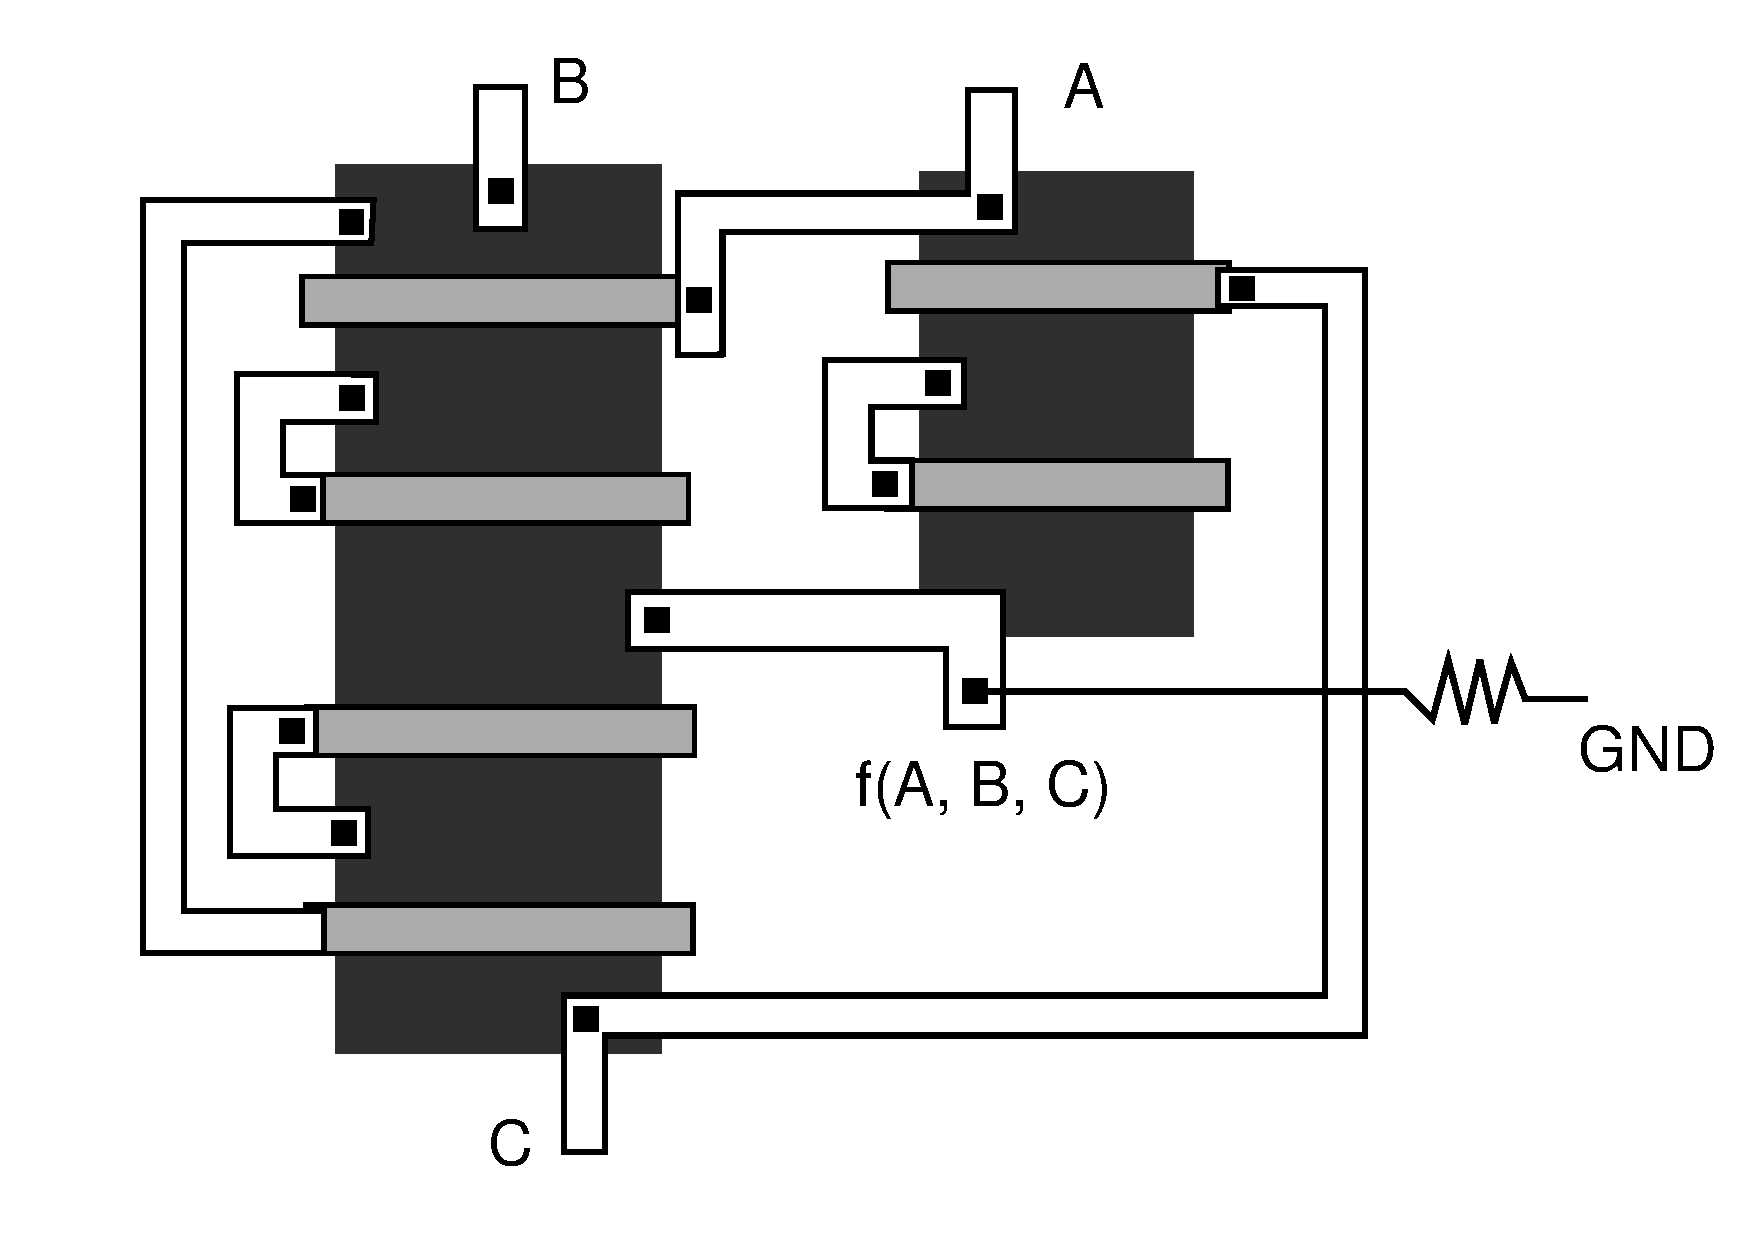
\includegraphics[width=0.7\textwidth]{fig/wafer.pdf}}
    \caption{The circuit (with short) from 
            Fig \ref{subfig:fetcircloop} on a wafer}
\label{fig:wafer}
\end{figure}

In figure, white represents wires, dark gray, the substrate, while
light gray represents the poly (gates). Note --- The diagram is meant to only be 
representative of positioning, so liberties have been taken with spacing
for the sake of clarity. 

